\documentclass[a4paper, 10pt, twoside]{article}

\usepackage[top=1in, bottom=1in, left=1in, right=1in]{geometry}
\usepackage[utf8]{inputenc}
\usepackage[spanish, es-ucroman, es-noquoting]{babel}
\usepackage{setspace}
\usepackage{fancyhdr}
\usepackage{lastpage}
\usepackage{amsmath}
\usepackage{amsfonts}
\usepackage{amsthm}
\usepackage{verbatim}
\usepackage{graphicx}
\usepackage{float}
\usepackage[noend]{algpseudocode}
\usepackage{enumitem} % Provee macro \setlist
\usepackage[toc, page]{appendix}


%%%%%%%%%% Configuración de Fancyhdr - Inicio %%%%%%%%%%
\pagestyle{fancy}
\thispagestyle{fancy}
\lhead{Trabajo Práctico 1 · Algoritmos y Estructuras de Datos III}
\rhead{Lovisolo · Petaccio · Rossi}
\renewcommand{\footrulewidth}{0.4pt}
\cfoot{\thepage /\pageref{LastPage}}

\fancypagestyle{caratula} {
   \fancyhf{}
   \cfoot{\thepage /\pageref{LastPage}}
   \renewcommand{\headrulewidth}{0pt}
   \renewcommand{\footrulewidth}{0pt}
}
%%%%%%%%%% Configuración de Fancyhdr - Fin %%%%%%%%%%


%%%%%%%%%% Configuración de Algorithmic - Inicio %%%%%%%%%%
% Entorno propio para customizar la presentación del pseudocódigo
\newenvironment{pseudo}[1][]{%
    \vspace{0.5em}%
    \begin{algorithmic}%
}
{%
    \end{algorithmic}%
    \vspace{0.5em}%
}

% Valores de verdad
\newcommand{\True}{\textbf{true}}
\newcommand{\False}{\textbf{false}}

% Conectivo 'in' para usar así: \ForAll{$foo$ \In $bar$}
\newcommand{\In}{\textbf{in} }

% Conectivo 'to' para usar así: \For{$i = 1$ \In $n$}
\newcommand{\To}{\textbf{to} }

% Complejidades
\newcommand{\Ode}[1]{\hfill $O(#1)$}
%%%%%%%%%% Configuración de Algorithmic - Fin %%%%%%%%%%


%%%%%%%%%% Miscelánea - Inicio %%%%%%%%%%
% Evita que el documento se estire verticalmente para ocupar el espacio vacío
% en cada página.
\raggedbottom

% Deshabilita sangría en la primer línea de un párrafo.
\setlength{\parindent}{0em}

% Separación entre párrafos.
\setlength{\parskip}{0.5em}

% Separación entre elementos de listas.
\setlist{itemsep=0.5em}

% Asigna la traducción de la palabra 'Appendices'.
\renewcommand{\appendixtocname}{Apéndices}
\renewcommand{\appendixpagename}{Apéndices}
%%%%%%%%%% Miscelánea - Fin %%%%%%%%%%


%%%%%%%%%% Gráficos - Inicio %%%%%%%%%%
% Macro para incluir tres gráficos (dentro de una figura) de manera que
% entren todos en una sola página.
\newcommand{\tresgraficos}[3]{
    \newcommand{\separacion}{-2.2em}
    \vspace{\separacion}
    \include{#1}
    \vspace{\separacion}
    \include{#2}
    \vspace{\separacion}
    \include{#3}
}
%%%%%%%%%% Gráficos - Fin %%%%%%%%%%


\begin{document}


%%%%%%%%%%%%%%%%%%%%%%%%%%%%%%%%%%%%%%%%%%%%%%%%%%%%%%%%%%%%%%%%%%%%%%%%%%%%%%%
%% Carátula                                                                  %%
%%%%%%%%%%%%%%%%%%%%%%%%%%%%%%%%%%%%%%%%%%%%%%%%%%%%%%%%%%%%%%%%%%%%%%%%%%%%%%%


\thispagestyle{caratula}

\begin{center}


\includegraphics[height=2cm]{DC.png} 
\hfill

\includegraphics[height=2cm]{UBA.jpg} 

\vspace{2cm}

Departamento de Computación,\\
Facultad de Ciencias Exactas y Naturales,\\
Universidad de Buenos Aires

\vspace{4cm}

\begin{Huge}
Trabajo Práctico 1
\end{Huge}

\vspace{0.5cm}

\begin{Large}
Algoritmos y Estructuras de Datos III
\end{Large}

\vspace{1cm}

Segundo Cuatrimestre de 2013

\vspace{4cm}

\begin{tabular}{|c|c|c|}
\hline
Apellido y Nombre & LU & E-mail\\
\hline
Leandro Lovisolo      & 645/11 & leandro@leandro.me\\
Lautaro José Petaccio & 443/11 & lausuper@gmail.com\\
Lucas Rossi           & 705/11 & lucasrossi20@gmail.com\\
\hline
\end{tabular}

\end{center}

\newpage


%%%%%%%%%%%%%%%%%%%%%%%%%%%%%%%%%%%%%%%%%%%%%%%%%%%%%%%%%%%%%%%%%%%%%%%%%%%%%%%
%% Índice                                                                    %%
%%%%%%%%%%%%%%%%%%%%%%%%%%%%%%%%%%%%%%%%%%%%%%%%%%%%%%%%%%%%%%%%%%%%%%%%%%%%%%%


\tableofcontents

\newpage


%%%%%%%%%%%%%%%%%%%%%%%%%%%%%%%%%%%%%%%%%%%%%%%%%%%%%%%%%%%%%%%%%%%%%%%%%%%%%%%
%% Introducción                                                              %%
%%%%%%%%%%%%%%%%%%%%%%%%%%%%%%%%%%%%%%%%%%%%%%%%%%%%%%%%%%%%%%%%%%%%%%%%%%%%%%%


\section{Introducción}

En el presente trabajo estudiamos tres problemas algorítmicos, proponemos soluciones para los mismos respetando sus requerimientos de complejidad temporal y analizamos empíricamente los tiempos de ejecución de sus implementaciones en lenguaje C++.

La motivación de este trabajo es comparar las cotas temporales obtenidas del análisis teórico con las mediciones de tiempos de ejecución y extraer conclusiones de esta experimentación.

Sin más, presentamos los problemas estudiados a continuación.


%%%%%%%%%%%%%%%%%%%%%%%%%%%%%%%%%%%%%%%%%%%%%%%%%%%%%%%%%%%%%%%%%%%%%%%%%%%%%%%
%% Problema 1: Pascual y el correo                                           %%
%%%%%%%%%%%%%%%%%%%%%%%%%%%%%%%%%%%%%%%%%%%%%%%%%%%%%%%%%%%%%%%%%%%%%%%%%%%%%%%


\newpage

\section{Problema 1: Pascual y el correo}

Dada una secuencia de paquetes y un límite de peso, se nos pide calcular, la cantidad de camiones necesarios y sus pesos, para realizar el transporte de los mismos, utilizando el método del encargado de logística llamado Pascual, el cuál consiste en lo siguiente:

\begin{itemize}
\item Si un paquete excede el peso del camión cargado con menor peso, se pide un nuevo camión y se coloca el paquete.
\item Si el paquete no supera el peso del camión cargado de menor peso, se lo coloca en el camión de menor peso.
\end{itemize}

Se nos pide resolver el problema con una cota de complejidad temporal \textbf{estrictamente mejor} que $O(n^2)$.

\textbf{Ejemplos del problema y sus soluciones:}

\textbf{Entrada}: límite: 100 , peso de paquetes: 3 80 40 60. \\
\textbf{Salida}: 2 80 100. \\
El camión 1 recibe el primer paquete de 80. Al intentar luego colocar el paquete de 40 en este, no le es posible debido a que el límite es 100 y lo guarda en el camión 2, al que luego, se le suma el paquete de 60, el cuál no provoca que el límite sea superado al colocarse en este.\\

\textbf{Entrada}: límite: 100, paquetes: 0.\\
\textbf{Salida}: 0. \\
Al no haber paquetes no se utilizan camiones, sin importar el límite del mismo.

\subsection{Solución}

Sea $\langle p_1, \ldots, p_n \rangle$ la secuencia que contiene los pesos de los $n$ paquetes en orden de llegada, sea $\langle c_1, \ldots, c_m \rangle$ la secuencia en orden ascendente que contiene las cargas de los camiones en un determinado momento (inicialmente vacía) y sea $L$ el límite de carga de los camiones.

Para cada paquete $p_i$, cargamos el paquete en el camión con menor carga $c_1$ si la nueva carga no supera el límite $L$, o en caso contrario agregamos un nuevo camión $c_{m+1} = p_i$ a la secuencia, realizando las permutaciones necesarias para preservar el orden ascendente.

Luego de haber cargado todos los paquetes, devolvemos la secuencia con la carga de cada camión.

Para cumplir con los requerimientos de complejidad temporal, utilizamos una cola de prioridad min-heap en lugar de una secuencia para almacenar las cargas de cada camión.

\begin{pseudo}
	\State Tipo de dato Camion es Tupla $\langle$ id : entero, carga : entero  $\rangle$
    \Procedure{Pascual-y-el-correo}{$\langle p_1, \ldots, p_n \rangle, L$}
        \State $C \leftarrow$ nuevo min-heap de Camion, ordenado por carga   \Ode{1}
        \ForAll{$p$ \In $\langle p_1, \ldots, p_n \rangle$}    	
            \If{$C.tama\tilde{n}o = 0$}                         \Ode{1}
                \State $C.encolar(\langle 1 , p \rangle)$       \Ode{log(n)}
            \ElsIf{$C.siguiente() + p \leq L$}                  \Ode{1}
                \State $c : Camion \leftarrow C.siguiente()$   \Ode{1}
                \State $c.carga \leftarrow c.carga + p$			\Ode{1}
                \State $C.desencolar()$                         \Ode{log(n)}
                \State $C.encolar(c)$                           \Ode{log(n)}
            \Else
                \State $C.encolar(\langle C.tama\tilde{n}o(), p \rangle)$ \Ode{log(n)}
            \EndIf
        \EndFor

  		\State $Camiones \leftarrow$ Arreglo de camiones de C.tamaño()
        \ForAll{$i$ \In $\langle 1, \ldots,$ C.tamaño() $\rangle$}			
      		\State Camiones[i] $\leftarrow$ $C.siguiente()$		\Ode{1}
      		\State $C.desencolar()$								\Ode{log(n)}
        \EndFor
        
        \State $Ordenar(Camiones)$ (Ordenamiento por id)		\Ode{log(n)}
        \State \textbf{return} $Camiones$
    \EndProcedure
\end{pseudo}


\subsection{Complejidad}

Para realizar el algoritmo se utilizó la estructura de datos priority\_queue que pertenece a la \textit{STL}.

Las operaciones operaciones utilizadas fueron \textit{top()} que corresponde a \textit{siguiente()} con complejidad \textit{O(1)} y \textit{push()} y \textit{pop()} que corresponden a \textit{encolar()} y \textit{desencolar()} con complejidad \textit{O(log(n))}.

El algoritmo corre en tiempo $O(n \times log(n))$, donde $n$ es la cantidad de paquetes.

\textbf{Demostración:} para cada uno de los $n$ paquetes, se realizan 1 ó 2 operaciones $O(log(n))$ sobre la cola de prioridad. Luego deducimos la complejidad total $n \times O(log(n)) = O(n \times log(n))$.


\subsection{Correctitud}
Sea m el paquete número m de la secuencia de paquetes recibida, con m-1 paquetes ubicados en camiones anteriormente, quiero ver si al ubicar el paquete m el algoritmo cumple con la metodología de ordenar paquetes de Pascual.

Al utilizar una \textbf{cola de prioridad} para almacenar los camiones, es posible asegurar que siempre se tendrá el camión menos cargado en cada llamada a \textbf{siguiente()}, corroborando el correcto funcionamiento de la consigna, la cuál describe que las comparaciones para elegir el destino del paquete se hacen con el camión de menor peso. 

Si la suma del peso del camión menor cargado (conseguido con \textbf{siguiente()}) y el nuevo paquete m no superan el límite, se procede a desencolar del heap el camión. Se le carga el nuevo paquete aumentando su peso y se lo encola nuevamente en el heap.Este se encargará de dejar el nuevo camión de menor carga disponible mediante \textbf{siguiente()}.

Si es requerido un nuevo camión, se crea uno nuevo con el peso del paquete m y se lo encola en el heap, nuevamente el heap se encargará de colocar el camión de menor peso de tal manera de estar disponible con \textbf{siguiente()}.

\subsection{Experimentos computacionales}
\subsubsection{Verificación de correctitud}
Elegimos los siguientes casos para verificar la correctitud del programa:
\begin{enumerate}
	\item Entrada vacía, verifica el comportamiento del algoritmo ante la posibilidad de no recibir ningún paquete en la entrada.
	\item Entrada con un único paquete, verifica el primer caso, el de tener el \textbf{min-heap} vacío.
	\item Entrada en la cual en algún camión se deba insertar más de un paquete. Esto verifica el caso del \textbf{else if} descripto en el pseudocódigo.
	\item Entrada en la cual algún camión no pueda contener el peso del nuevo paquete y deba pedir un nuevo camión. Esto verifica el caso final (\textbf{else}), debiendo incluir un nuevo camión.
\end{enumerate}


\subsubsection{Performance}

Previo a los experimentos realizados suponíamos que el peor caso sería cuando el tamaño de los paquetes sea igual al límite de los camiones, pero al realizarlos pudimos concluir que ese caso es el peor para Pascual, ya que tiene que utilizar una mayor cantidad de camiones y que el peor caso es cuando los paquetes están ordenados en forma decreciente, ya que se utiliza un min-heap como estructura y el camión a insertar tiene el peso mínimo
deberá reordenarse hasta llegar a la cabecera del heap realizando la mayor cantidad de operaciones posibles para la inserción.

Concluimos también en que tener una sucesión de paquetes, los cuales entren todos en un solo camión, determina el mejor caso. Esto se debe a que sólo es necesaria la primera inserción en el heap, que como este es vacío es O(1) y luego no se utilizan otras operaciones sobre el heap que no sean O(1) (siguiente()) ya que sólo se carga un solo camión. Lo que lleva a tener una complejidad de $\Omega(n)$.

Para los experimentos aleatorios se generaron n paquetes, donde el peso de cada uno se generó mediante un entero aleatorio con valor entre 0 y el límite de peso de los camiones, con distribución uniforme. 

\subsubsection{Peor caso}

\begin{figure}[H]
  \centering
  \tresgraficos{problema1-peor-caso}
               {problema1-peor-caso-logn}
               {problema1-peor-caso-n}               
  \caption{Peor caso}
\end{figure}


\subsubsection{Mejor caso}

\begin{figure}[H]
  \centering
  \tresgraficos{problema1-mejor-caso}
               {problema1-mejor-caso-logn}
               {problema1-mejor-caso-n}
  \caption{Mejor caso}
\end{figure}


\subsubsection{Instancias aleatorias}

\begin{figure}[H]
  \centering
  \tresgraficos{problema1-instancias-aleatorias}
               {problema1-instancias-aleatorias-logn}
               {problema1-instancias-aleatorias-n}
  \caption{Instancias aleatorias}
\end{figure}


%%%%%%%%%%%%%%%%%%%%%%%%%%%%%%%%%%%%%%%%%%%%%%%%%%%%%%%%%%%%%%%%%%%%%%%%%%%%%%%
%% Problema 2: Profesores visitantes                                         %%
%%%%%%%%%%%%%%%%%%%%%%%%%%%%%%%%%%%%%%%%%%%%%%%%%%%%%%%%%%%%%%%%%%%%%%%%%%%%%%%


\newpage

\section{Problema 2: Profesores visitantes}

Dado un conjunto de $n$ cursos con una fecha de inicio y una fecha de finalización, se nos pide hallar el subconjunto con mayor cantidad de cursos tales que ningún curso se solapa con otro.

Se representa cada curso con una tupla $(i, f)$, donde $i$ y $f$ son las fechas de inicio y finalización del curso, respectivamente, tales que $i \leq f$.

Decimos que dos cursos $(i_1, f_1)$ y $(i_2, f_2)$ con $f_1 \leq f_2$ se solapan si y sólo si $f_1 \geq i_2$.

Formalmente, dado un conjunto de cursos $C = \{ (i_1, f_1), \ldots, (i_n, f_n) \}$, se nos pide hallar un subconjunto $S \subseteq C$ sin cursos solapados, tal que para cualquier otro $S' \subseteq C$ sin cursos solapados, vale que $|S| \geq |S'|$.

El problema debe ser resuelto con una cota de complejidad temporal \textbf{estrictamente mejor} que $O(n^2)$.

Algunas instancias del problema y sus soluciones:

\textbf{Entrada}: $\{(4, 4), (1, 3), (2, 5)\}$.\\
\textbf{Salida}: $\{(1, 3), (4, 4)\}$.

\textbf{Entrada}: $\{(4, 10), (5, 6), (2, 3), (7, 8), (3, 4), (1, 15)\}$.\\
\textbf{Salida}: $\{(2, 3), (5, 6), (7, 8)\}$ ó $\{(3, 4), (5, 6), (7, 8)\}$; cualquiera de las dos son correctas.

\textbf{Entrada}: $\{(1, 2)\}$.\\
\textbf{Salida}: $\{(1, 2)\}$.

\textbf{Entrada}: $\emptyset$.\\
\textbf{Salida}: $\emptyset$.


\subsection{Solución}

Sea $C = \{ (i_1, f_1), \ldots, (i_n, f_n) \}$ el conjunto con los $n$ cursos ordenados por fecha de finalización en forma creciente ($i < j \Rightarrow f_i \leq f_j$), y sea $S = \emptyset$ una solución del problema, inicialmente vacía.

Recorremos los cursos $c_j \in C$ (con $j = 1, \ldots, n$) en el orden anterior, realizando una de las siguientes acciones para cada $c_j$:

\begin{itemize}
    \item{
        Si $j = 1$, incluímos $c_1 = (i_1, f_1)$ en la solución: $S = \{ (i_1, f_1) \}$.
    }
    \item{
        Si $j > 1$ y $c_j = (i_j, f_j)$ \textbf{no se solapa} con el último curso agregado a la solución, lo incluímos en la misma: $S = S \cup \{ (i_j, f_j) \}$.
    }
    \item{
        En caso contrario, ignoramos $c_j$.
    }
\end{itemize}

Finalmente devolvemos la solución $S$ hallada.

En el pseudocódigo a continuación, $C$ denota el conjunto con la oferta de $n$ cursos $\{ (i_1, f_1), \ldots, (i_n, f_n) \}$.

\begin{pseudo}
    \Procedure{Profesores-visitantes}{$C$}
        \If{$|C| < 2$}
            \State{\Return{$C$}}                                \Ode{1}
        \Else
            \State{Ordenar $C$ por fecha de finalización
                   en forma creciente.}                         \Ode{n \times log(n)}
            \State{$S = \{(i_1, j_1)\}$}                        \Ode{1}
            \State{$k = 1$}                                     \Ode{1}
            \For{$j = 2$ \To $|C|$}                            
                \If{$i_j > f_k$}                                \Ode{1}
                    \State{$S = S \cup \{ (i_j, f_j) \}$}       \Ode{1}
                    \State{$k = j$}                             \Ode{1}
                \EndIf
            \EndFor
            \State{\Return{$S$}}
        \EndIf
    \EndProcedure 
\end{pseudo}


\subsection{Complejidad}

El algoritmo corre en tiempo $O(n \times log(n))$, donde $n$ es la cantidad de cursos.

\begin{proof}
    Para el caso no trivial ($n > 1$) se ordenan los cursos en $O(n \times log(n))$, luego se recorre cada curso y se decide si se lo incluye en la solución o no, con costo $n \times O(1)$. La complejidad total resulta $O(n \times log(n)) + n \times O(1) = O(n \times log(n) + n) = O(n \times log(n))$. Para el caso trivial, se devuelve el conjunto de cursos intacto en tiempo constante.
\end{proof}


\subsection{Correctitud}

El algoritmo incluye en la solución el curso que termina primero, descarta los cursos que se solapan con este y repite lo anterior con los cursos restantes hasta que no queden más cursos.

Para que el procedimiento anterior arroje una solución válida, tiene que cumplirse que para cualquier instancia del problema, el curso con fecha de finalización más temprana siempre sea parte de alguna solución. Si esto se cumple, podemos incluir dicho curso en nuestra solución, descartar todos los cursos que se solapan con este, resolver el subproblema resultante aplicando el mismo razonamiento e incluir la solución del subproblema en la solución al problema original.

El teorema a continuación muestra que la suposición anterior es de hecho cierta.

\newtheorem*{teorema-ej2}{Teorema}

\begin{teorema-ej2}
    Sea $C = \{ (i_1, f_1), \ldots, (i_n, f_n) \}$ la oferta de $n$ cursos ordenados por fecha de finalización de forma creciente. Entonces el curso $(i_1, f_1)$ está incluido en algún subconjunto de $C$ tal que sus cursos no se solapan entre sí y su cardinalidad es máxima.
\end{teorema-ej2}

\begin{proof}
    Sea $S$ algún subconjunto $\subseteq C$ tal que sus cursos no se solapan entre sí y su cardinalidad es máxima, y sea $(i_j, f_j)$ el curso $\in S$ con fecha de finalización más temprana.

    Si $(i_j, f_j) = (i_1, f_1)$ terminamos la demostración, pues hemos mostrado que $(i_1, f_1)$ está incluido en algún subconjunto de $C$ tal que sus cursos no se solapan entre sí y su cardinalidad es máxima.

    Si $(i_j, f_j) \neq (i_1, f_1)$, entonces sea $S' = S - \{ (i_j, f_j) \} \cup \{ (i_1, f_1) \}$ el conjunto $S$ al que le reemplazamos $(i_j, f_j)$ por $(i_1, f_1)$. Los cursos en $S'$ no se solapan entre sí pues:

    \begin{itemize}[nolistsep]
        \item{los cursos en $S$ no se solapan entre sí,}
        \item{$(i_j, f_j)$ es la actividad en $S$ que termina primero, y}
        \item{$f_1 \leq f_j$.}
    \end{itemize}

    Como $|S'| = |S|$, concluímos que $S'$ es un subconjunto de $C$ tal que sus cursos no se solapan entre sí y su cardinalidad es máxima, y $(i_1, f_1)$ está incluido en $S'$, como queríamos ver.
\end{proof}


\subsection{Experimentos computacionales}

\subsubsection{Verificación de correctitud}

Elegimos los siguientes casos de prueba para verificar la correctitud del programa:

\begin{enumerate}
\item Entrada vacía, verficia el comportamiento del algoritmo ante una entrada vacía.
\item Entrada con un único curso, verifica el caso de tener como entrada y solución un único curso.
\item Entrada en la cuál dos cursos se solapen, verifica el caso en el que el algoritmo deberá descartar el curso que solapa al otro.
\item Entrada en la cuál existan cursos que no se solapen, verifica el caso en el que dos o más cursos puedan cohexistir en un cronograma.
\end{enumerate}

\subsubsection{Performance}
Medimos experimentalmente la performance del algoritmo para instancias aleatorias, del mejor y peor caso; de tamaños $1, \ldots, 1000$.

Dado que la operación de ordenamiento de los cursos domina la complejidad del problema, tomamos como mejor y peor caso los respectivos casos del algoritmo de ordenamiento; es decir, cuando el vector ya está ordenado y cuando el vector está en el orden inverso, respectivamente.

En nuestra implementación utilizamos el algoritmo de ordenamiento provisto en la librería estándar de C++, que garantiza una cota de complejidad $O(n \times log(n))$, pero no menciona explícitamente sus casos mejor y peor. Los casos mejor y peor que tomamos fueron decididos a partir de nuestro conocimiento teórico de algoritmos de sorting.

Los cursos de las instancias aleatorias fueron generadas tomando dos enteros aleatorios con distribución uniforme en el intervalo $0, \ldots, 999$ como fechas de inicio y finalización, tales que la fecha de inicio es menor o igual a la de finalización.

\subsubsection{Peor caso}

\begin{figure}[H]
  \centering
  \tresgraficos{problema2-peor-caso}
               {problema2-peor-caso-logn}
               {problema2-peor-caso-n}               
  \caption{Peor caso}
\end{figure}


\subsubsection{Mejor caso}

\begin{figure}[H]
  \centering
  \tresgraficos{problema2-mejor-caso}
               {problema2-mejor-caso-logn}
               {problema2-mejor-caso-n}
  \caption{Mejor caso}
\end{figure}


\subsubsection{Instancias aleatorias}

\begin{figure}[H]
  \centering
  \tresgraficos{problema2-instancias-aleatorias}
               {problema2-instancias-aleatorias-logn}
               {problema2-instancias-aleatorias-n}
  \caption{Instancias aleatorias}
\end{figure}


%%%%%%%%%%%%%%%%%%%%%%%%%%%%%%%%%%%%%%%%%%%%%%%%%%%%%%%%%%%%%%%%%%%%%%%%%%%%%%%
%% Problema 3: Una noche en el museo                                         %%
%%%%%%%%%%%%%%%%%%%%%%%%%%%%%%%%%%%%%%%%%%%%%%%%%%%%%%%%%%%%%%%%%%%%%%%%%%%%%%%


\newpage

\section{Problema 3: Una noche en el museo}
Se desea instalar un sistema de detección de movimientos basado en sensores láser, para esto cada piso del museo fue modelado por una grilla de $n$ $x$ $m$ casillas.

Existen dos tipos de sensores, bidireccionales (emiten señales hacia la izquierda y la derecha o bien hacia arriba y abajo) y cuatridireccionales (emiten señales en las 4 direcciones), de \$4000 y \$6000 respectivamente y 3 tipos de casilla, vacía, importante y pared.

Dado un piso se debe cumplir:

\begin{itemize}
\item las casillas libres deben quedar cubiertas por al menos un sensor.
\item las casilla importantes deben ser cubiertas por dos sensores.
\item no se puede ubicar un sensor de forma tal que alguna de sus señales impacten contra otro dispositivo.
\item no se puede instalar más de un dispositivo en una misma casilla libre.
\item en caso de haber solución, la misma debrá minimizar la cantidad de dinero invertido en sensores.
\end{itemize}

Se pide realizar el algoritmo mediante la técnica de Backtracking.

\textbf{Ejemplo:}
\begin{figure}[H]
  \centering
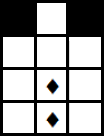
\includegraphics[width=0.20\textwidth]{ejemplo_problema3/grilla.png}
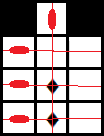
\includegraphics[width=0.20\textwidth]{ejemplo_problema3/grilla-sol16000.png}
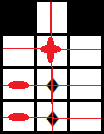
\includegraphics[width=0.20\textwidth]{ejemplo_problema3/grilla-sol14000.png}
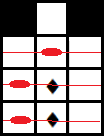
\includegraphics[width=0.20\textwidth]{ejemplo_problema3/grillaSinSol.png}
  \caption{Instacia del problema, dos soluciones distintas con un costo de \$14.000 y \$16.000 respectivamente y una solución no válida} 
  \label{fig:1}
\end{figure}


\subsection{Solución}

% Posiciones posibles
\newcommand{\Libre}{\texttt{Libre}}
\newcommand{\Sensado}{\texttt{Sensado}}
\newcommand{\Importante}{\texttt{Importante}}
\newcommand{\Pared}{\texttt{Pared}}
\newcommand{\SensorV}{\texttt{SensorVertical}}
\newcommand{\SensorH}{\texttt{SensorHorizontal}}
\newcommand{\SensorC}{\texttt{SensorCuadruple}}

Representamos un piso $P$ como una matriz de $m$ filas por $n$ columnas, donde cada $p_{ij} \in P$ tiene cualquiera de los siguientes valores: \Libre, \Sensado, \Importante, \Pared, \SensorV, \SensorH, \SensorC.

Dado un piso $P$ sin sensores, recorremos el árbol de combinaciones de sensores posibles en búsqueda de una solución óptima de la siguiente manera:

\begin{enumerate}
    \item{
        \label{buscar-posicion-libre}
        Buscamos la primera posición libre $(i, j)$ recorriendo el piso de izquierda a derecha y de arriba a abajo, partiendo de la esquina superior izquierda.

        \begin{pseudo}
            \State $i \leftarrow 1$, $j \leftarrow 1$             \Ode{1}
            \While{$i \leq m \land p_{ij} \neq \Libre$}           \Ode{m \times n}
                \If{$j < n$}                                      \Ode{1}
                    \State $j \leftarrow j + 1$                   \Ode{1}
                \Else                                             \Ode{1}
                    \State $i \leftarrow i + 1$, $j \leftarrow 1$ \Ode{1}
                \EndIf
            \EndWhile
        \end{pseudo}

         Si no encontramos ninguna posición libre (es decir, si $i > m$), saltamos al paso \ref{ultimo-paso}.
    }
    \item{
        \label{generar-pisos}
        Generamos 4 pisos nuevos, copiando el piso $P$ y:
        \begin{enumerate}
            \item{
                Poniendo un sensor vertical en $(i, j)$. \Ode{m \times n}
            }
            \item{
                Poniendo un sensor horizontal en $(i, j)$. \Ode{m \times n}
            }
            \item{
                Poniendo un sensor cuádruple en $(i, j)$. \Ode{m \times n}
            }
            \item{
                \label{posicion-libre}
                Dejando libre la posición $(i, j)$ (es decir, este nuevo piso es idéntico al piso $P$.) \Ode{m \times n}
            }
        \end{enumerate}
    }
    \item{
        Para cada piso $Q$ generado en el paso anterior, marcamos como sensadas todas las posiciones libres afectadas por el nuevo sensor (no aplica para el caso \ref{posicion-libre}.)

        \begin{pseudo}
            \If{$q_{ij} \in \{ \SensorV, \SensorC \}$}                                   \Ode{m}
                \For{$i'$ \In $\textsc{Columna-Visible}(q_{ij})$}                        \Ode{m}
                    \State $q_{i'j} \leftarrow \Sensado$ \textbf{if} $q_{i'j} = \Libre$  \Ode{1}
                \EndFor
            \EndIf
            \If{$q_{ij} \in \{ \SensorH, \SensorC \}$}                                   \Ode{n}
                \For{$j'$ \In $\textsc{Fila-Visible}(q_{ij})$}                           \Ode{n}
                    \State $q_{ij'} \leftarrow \Sensado$ \textbf{if} $q_{ij'} = \Libre$  \Ode{1}
                \EndFor
            \EndIf
        \end{pseudo}

        \begin{pseudo}
            \Procedure{Fila-Visible}{$q_{ij}$}                            \Ode{n}
                \State $C \leftarrow \{ j \}$                             \Ode{n}
                \For{$rango$ \In $\{ (j, \ldots, 1), (j, \ldots, n)  \}$} \Ode{2 \times n}
                    \For{$j'$ \In $rango$}                                \Ode{n}
                        \State \textbf{break if} $q_{ij'} = \Pared$       \Ode{1}
                        \State $C \leftarrow C \cup \{ j' \}$             \Ode{1}
                    \EndFor
                \EndFor
                \State \Return{$C$}                                       \Ode{1}
            \EndProcedure
        \end{pseudo}

        \begin{pseudo}
            \Procedure{Columna-Visible}{$q_{ij}$}                         \Ode{m}
                \State $F \leftarrow \{ i \}$                             \Ode{1}
                \For{$rango$ \In $\{ (i, \ldots, 1), (i, \ldots, m)  \}$} \Ode{2 \times m}
                    \For{$i'$ \In $rango$}                                \Ode{m}
                        \State \textbf{break if} $q_{i'j} = \Pared$       \Ode{1}
                        \State $F \leftarrow F \cup \{ i' \}$             \Ode{1}
                    \EndFor
                \EndFor
                \State \Return{$F$}                                       \Ode{1}
            \EndProcedure
        \end{pseudo}
    }
    \item{
        Para cada piso $Q$ resultante del paso anterior, descartamos los que correspondan según el criterio de poda (ver \textit{Podas} más abajo.)
    }
    \item{
        \label{paso-recursivo}
        Para cada piso $Q$ que no fue descartado en el paso anterior:
        \begin{enumerate}
            \item{
                Buscamos la siguiente posición libre $(i', j')$ de la misma manera que en el paso \ref{buscar-posicion-libre}, pero partiendo de $(i, j+1)$ en vez de la esquina superior izquierda, ó $(i+1, 1)$ si $j=n$. \Ode{m \times n}
            }
            \item{
                Si encontramos una posición libre, repetimos los pasos $\ref{generar-pisos}, \ldots, \ref{paso-recursivo}$ utilizando $Q$ en lugar de $P$, y $(i', j')$ en lugar de $(i, j)$.
            }
            \item{
                \label{decidir-si-es-solucion}
                En caso contrario, decidimos si el piso es solución.

                \begin{pseudo}
                    \State $esSolucion \leftarrow \True$                                       \Ode{1}
                    \For{$i$ \In $1, \ldots, m$, $j$ \In $1, \ldots, n$}                       \Ode{m \times n \times (m + n)}
                        \If{$q_{ij} = \Importante$}                                            \Ode{m + n}
                            \State $s \leftarrow \textsc{\#-Sensores-Actuando-Sobre}(q_{ij})$  \Ode{m + n}
                        \EndIf

                        \If{$q_{ij} = \Libre$ $\lor$ $(q_{ij} = \Importante$ $\land$ $s < 2)$} \Ode{1}
                            \State $esSolucion \leftarrow \False$                              \Ode{1}
                            \State \textbf{break}
                        \EndIf
                    \EndFor
                \end{pseudo}

                \begin{pseudo}
                    \Procedure{\#-Sensores-Actuando-Sobre}{$q_{ij}$}      \Ode{m + n}
                        \State $s \leftarrow 0$                           \Ode{1}
                        \For{$i'$ \In $\textsc{Columna-Visible}(q_{ij})$} \Ode{m}
                            \If{$q_{i'j} \in \{ \SensorV, \SensorC \}$}   \Ode{1}
                                \State $s \leftarrow s + 1$               \Ode{1}
                                \State \textbf{break}
                            \EndIf
                        \EndFor
                        \For{$j'$ \In $\textsc{Fila-Visible}(q_{ij})$}    \Ode{n}
                            \If{$q_{ij'} \in \{ \SensorH, \SensorC \}$}   \Ode{1}
                                \State $s \leftarrow s + 1$               \Ode{1}
                                \State \textbf{break}
                            \EndIf
                        \EndFor
                        \State \Return{$s$}                               \Ode{1}
                    \EndProcedure
                \end{pseudo}


            }
            \item{
                Si es solución y es más barata que la mejor solución $S$ hallada hasta el momento, o si aún no se halló ninguna solución, la marcamos como mejor solución.

                \begin{pseudo}
                    \If{$esSolucion$}
                        \If{$S = \textbf{nil}$ $\lor$ $\textsc{Costo}(Q) < \textsc{Costo}(S)$} \Ode{m \times n}
                            \State $S \leftarrow Q$ (referencia)                               \Ode{1}
                        \EndIf
                    \EndIf
                \end{pseudo}

                \begin{pseudo}
                    \Procedure{Costo}{$Q$}                                            \Ode{m \times n}
                        \State $c \leftarrow 0$                                       \Ode{1}
                        \For{$i$ \In $1, \ldots, m$, $j$ \In $1, \ldots, n$}          \Ode{m \times n}
                            \State $c \leftarrow c + 4000$
                                    \textbf{if} $q_{ij} \in \{ \SensorV, \SensorH \}$ \Ode{1}
                            \State $c \leftarrow c + 6000$
                                \textbf{if} $q_{ij} = \SensorC$                       \Ode{1}
                        \EndFor
                        \State \Return{$c$}                                           \Ode{1}
                    \EndProcedure
                \end{pseudo}                
            }
        \end{enumerate}
    }
    \item{
        \label{ultimo-paso}
        Devolvemos la mejor solución hallada $S$, que puede ser \textbf{nil} en caso de no haberse hallado una.
    }
\end{enumerate}


\subsubsection{Podas}

Las podas a continuación se realizan siempre para cada piso $Q$ generado en el paso \ref{generar-pisos}, donde $q_{ij}$ es la posición que se modificó (o se dejó intacta en el caso \ref{posicion-libre}) luego de copiar el piso $P$ original.

Si $q_{ij} \in \{ \SensorV, \SensorH, \SensorC \}$:

\begin{enumerate}
    \item{
        \label{poda-sensores-incompatibles}
        Si $q_{ij} \in \{ \SensorV, \SensorH, \SensorC \}$, podamos si su señal impacta otro sensor o viceversa; es decir, si $\textsc{Impacta-Otro-Sensor}(q_{ij}) = \True$.

        \begin{pseudo}
            \Procedure{Impacta-Otro-Sensor}{$q_{ij}$}                       \Ode{m + n}
                \For{$i'$ \In $\textsc{Columna-Visible}(q_{ij})$}           \Ode{m}
                    \If{$\textsc{Sensores-Incompatibles}(q_{ij}, q_{i'j})$} \Ode{1}
                        \State \Return{\True}                               \Ode{1}
                    \EndIf
                \EndFor
                \For{$j'$ \In $\textsc{Fila-Visible}(q_{ij})$}              \Ode{n}
                    \If{$\textsc{Sensores-Incompatibles}(q_{ij}, q_{ij'})$} \Ode{1}
                        \State \Return{\True}                               \Ode{1}
                    \EndIf
                \EndFor
                \State \Return{\False}                                      \Ode{1}
            \EndProcedure
        \end{pseudo}

        \begin{pseudo}
            \Procedure{Sensores-Incompatibles}{$q_{ij}, q_{i'j'}$}     \Ode{1}
                \If{$i = i'$}                                          \Ode{1}
                    \If{$\textsc{Sensa-Horizontalmente}(q_{ij}) \lor
                            \textsc{Sensa-Horizontalmente}(q_{i'j'})$} \Ode{1}
                        \State \Return{\True}                          \Ode{1}
                    \EndIf
                \EndIf
                \If{$j = j'$}                                          \Ode{1}
                    \If{$\textsc{Sensa-Verticalmente}(q_{ij}) \lor
                            \textsc{Sensa-Verticalmente}(q_{i'j'})$}   \Ode{1}
                        \State \Return{\True}                          \Ode{1}
                    \EndIf
                \EndIf
                \State \Return{\False}                                 \Ode{1}
            \EndProcedure
        \end{pseudo}

        \begin{pseudo}
            \Procedure{Sensa-Verticalmente}{$q_{ij}$}                 \Ode{1}
                \State \Return{$q_{ij} \in \{ \SensorV, \SensorC \}$} \Ode{1}
            \EndProcedure
        \end{pseudo}

        \begin{pseudo}
            \Procedure{Sensa-Horizontalmente}{$q_{ij}$}               \Ode{1}
                \State \Return{$q_{ij} \in \{ \SensorH, \SensorC \}$} \Ode{1}
            \EndProcedure
        \end{pseudo}
    }
    \item{
        \label{poda-produce-posiciones-insensables}
        Si $q_{ij} \in \{ \SensorV, \SensorH \}$, podamos si produce que una posición libre en su misma fila o columna sea imposible de sensar.

        Esto ocurre cuando existe un sensor vertical y un sensor horizontal en la misma fila y columna de una posición libre, respectivamente, y no hay una pared entre los sensores y esa posición.

        \begin{pseudo}
            \State $podar \leftarrow \False$                                           \Ode{1}
            \If{$q_{ij} = \SensorV$}                                                   \Ode{m \times n}
                \For{$j'$ \In $\textsc{Fila-Visible}(q_{ij})$}                         \Ode{m \times n}
                    \If{$q_{ij'} = \Libre \land
                            \textsc{Hay-Un-Sensor-Horizontal-En-Su-Columna}(q_{ij'})$} \Ode{m}
                        \State $podar \leftarrow \True$                                \Ode{1}
                        \State \textbf{break}
                    \EndIf
                \EndFor
            \EndIf
            \If{$q_{ij} = \SensorH$}                                                   \Ode{1}
                \For{$i'$ \In $\textsc{Columna-Visible}(q_{ij})$}                      \Ode{m \times n}
                    \If{$q_{i'j} = \Libre \land
                            \textsc{Hay-Un-Sensor-Vertical-En-Su-Fila}(q_{i'j})$}      \Ode{n}
                        \State $podar \leftarrow \True$                                \Ode{1}
                        \State \textbf{break}
                    \EndIf
                \EndFor
            \EndIf
            \State Podamos $Q$ si $podar = \True$.
        \end{pseudo}

        \begin{pseudo}
            \Procedure{Hay-Un-Sensor-Horizontal-En-Su-Columna}{$q_{ij}$} \Ode{m}
                \For{$i'$ \In $\textsc{Columna-Visible}(q_{ij})$}        \Ode{m}
                    \If{$q_{i'j} = \SensorH$}                            \Ode{1}
                        \State \Return{\True}                            \Ode{1}
                    \EndIf
                \EndFor
                \State \Return{\False}                                   \Ode{1}
            \EndProcedure
        \end{pseudo}

        \begin{pseudo}
            \Procedure{Hay-Un-Sensor-Vertical-En-Su-Fila}{$q_{ij}$} \Ode{n}
                \For{$j'$ \In $\textsc{Fila-Visible}(q_{ij})$}      \Ode{n}
                    \If{$q_{ij'} = \SensorV$}                       \Ode{1}
                        \State \Return{\True}                       \Ode{1}
                    \EndIf
                \EndFor
                \State \Return{\False}                              \Ode{1}
            \EndProcedure
        \end{pseudo}
    }
    \item{
        \label{poda-costo}
        Si $q_{ij} \in \{ \SensorV, \SensorH, \SensorC \}$, podamos si el costo del piso supera o iguala el de la mejor solución $S$ hallada hasta el momento; es decir, si $\textsc{Costo}(Q) \geq \textsc{Costo}(S)$.
        \Ode{m \times n}
    }

    \item{
        \label{poda-posicion-insensable}
        Si $q_{ij} = \Libre$, podamos si $q_{ij}$ es imposible de sensar.

        Esto ocurre cuando no existe otra posición libre en su misma fila o columna sin una pared entre ambas, tal que se pueda poner un sensor apuntando a la misma, sin que su señal impacte otros sensores o viceversa.

        \begin{pseudo}
            \State $podar \leftarrow \True$                               \Ode{1}
            \For{$i'$ \In $\textsc{Columna-Visible}(q_{ij})$}             \Ode{m^2 \times n}
                \If{$q_{i'j} = \Libre$}                                   \Ode{m \times n}
                    \State $R \leftarrow Q$ (copia)                       \Ode{m \times n}
                    \State $r_{i'j} \leftarrow \SensorV$                  \Ode{1}
                    \If{$\textsc{Impacta-Otro-Sensor}(r_{i'j}) = \False$} \Ode{m + n}
                        \State $podar \leftarrow \False$                  \Ode{1}
                    \EndIf
                \EndIf
            \EndFor
            \For{$j'$ \In $\textsc{Fila-Visible}(q_{ij})$}                \Ode{m \times n^2}
                \If{$q_{ij'} = \Libre$}                                   \Ode{m \times n}
                    \State $R \leftarrow Q$ (copia)                       \Ode{m \times n}
                    \State $r_{ij'} \leftarrow \SensorV$                  \Ode{1}
                    \If{$\textsc{Impacta-Otro-Sensor}(r_{ij'}) = \False$} \Ode{m + n}
                        \State $podar \leftarrow \False$                  \Ode{1}
                    \EndIf
                \EndIf
            \EndFor
            \State Podamos $Q$ si $podar = \True$.
        \end{pseudo}

        Nota: el costo total de esta poda es $O(m^2 \times n) + O(m \times n^2) = O(m \times n \times (m + n))$.
    }
\end{enumerate}


\subsection{Complejidad}

El algoritmo corre en tiempo $O(4^p \times m \times n \times (m + n))$, donde $m$ es la cantidad de filas del piso, $n$ es la cantidad de columnas del piso y $p$ es la cantidad de posiciones libres en el piso.

\begin{proof}
    El algoritmo compara entre $O(4^p)$ pisos posibles, pues para cada posición libre existen 4 posibilidades: dejarla libre o poner un sensor vertical, horizontal o cuádruple; y de no realizar de ninguna poda, esto generaría $4^p$ combinaciones posibles.

    Para cada piso evaluado, se realizan la siguiente secuencia de operaciones:

    \begin{itemize}
        \item{Se genera una copia del piso original, con costo $O(m \times n)$.}
        \item{Se ubica un sensor en la posición designada y se marcan como sensadas las posiciones afectadas por este, con costo $O(m + n)$. Alternativamente, se deja libre esa posición, con costo $O(1)$.}
        \item{
            Si se agregó un nuevo sensor:
            \begin{itemize}
                \item{Se evalúa la poda \ref{poda-sensores-incompatibles}, con costo $O(m + n)$.}
                \item{Se evalúa la poda \ref{poda-produce-posiciones-insensables}, con costo $O(m \times n)$.}
                \item{Se evalúa la poda \ref{poda-costo}, con costo $O(m \times n)$.}
            \end{itemize}
        }
        \item{En caso contrario, se evalúa la poda \ref{poda-posicion-insensable}, con costo $O(m \times n \times (m + n))$.}
        \item{Se busca la siguiente posición libre, con costo $O(m \times n)$.}
        \item{Si se encontró una posición libre, terminamos de procesar el piso actual y continuamos con los 4 pisos resultantes de evaluar cada posibilidad para la posición libre hallada, con costo $O(1)$.}
        \item{
            Si no se encontró una posición libre:
            \begin{itemize}
                \item{Se verifica si el piso es solución, con costo $O(m \times n \times (m + n))$.}
                \item{Si es solución, se verifica si es óptima, con costo $O(m \times n)$.}
            \end{itemize}
        }
    \end{itemize}

    El costo total por piso está acotado por $O(m \times n \times (m + n))$ pues es el costo de la poda más costosa. Las demás podas tienen costo menor, y por lo tanto respetan esta cota. El resto de las operaciones en la secuencia tiene costo menor o igual.

    Finalmente, el costo total está dado por el producto entre la cantidad de pisos evaluados y el costo por piso, es decir $O(4^p) \times O(m \times n \times (m + n)$, que es equivalente a $O(4^p \times m \times n \times (m + n))$.
\end{proof}


\subsection{Correctitud}

Para probar que nuestro algoritmo es correcto, debe valer lo siguiente:

\begin{enumerate}
    \item{El algoritmo evalúa todo el espacio de pisos posibles.}
    \item{Sólo podamos ramas que conduzcan a soluciones subóptimas, o a pisos que no son solución.}
    \item{Se evalúan todas las soluciones que superan los criterios de poda.}
    \item{La solución devuelta es la óptima.}
\end{enumerate}


\subsubsection{El algoritmo evalúa todo el espacio de pisos posibles}

\begin{proof}
    El algoritmo recibe un piso con $p$ posiciones libres, el cual está asociado a un espacio de $4^p$ combinaciones de sensores posibles. Toma la primera posición libre y evalúa los 4 pisos resultantes de ubicar en esa posición cada uno de los tres sensores posibles o de dejarla intacta.

    Cada uno de estos pisos genera $4^{p-1}$ subproblemas posibles. En el supuesto caso que no se podara ninguno, esto generaría 4 pisos con $4^{p-1}$ subproblemas cada uno; es decir, un total de $4 \times 4^{p-1}$ subproblemas, que es igual a la cantidad de subproblemas original: $4^p$.

    Aplicando este razonamiento para cada subproblema, recorremos recursivamente el árbol de subproblemas, evaluando subárboles cada vez más chicos, hasta eventualmente alcanzar los $4^p$ subproblemas hoja (o una cantidad menor en caso de haber realizado podas.)

    Si bien el algoritmo no necesariamente recorre los $4^p$ pisos posibles, este \textbf{evalúa} las $4^p$ posibilidades distintas al tomar una decisión sobre si proceder por cada rama del árbol o no.
\end{proof}


\subsubsection{Sólo podamos ramas que conduzcan a soluciones subóptimas, o a pisos que no son solución}

\begin{proof}
    La poda \ref{poda-sensores-incompatibles} descarta un piso si la señal del nuevo sensor impacta otro sensor o viceversa. Si esto ocurre, el piso no es solución, pues es una condición prohibida por definición. A su vez, cualquier subproblema dentro de esta rama tampoco es solución, pues sólo se modifican las posiciones libres y los dos sensores incompatibles permanecen en conflicto.

    La poda \ref{poda-produce-posiciones-insensables} descarta un piso si el nuevo sensor produce que alguna posición $(i, j)$ sea imposible de sensar; es decir, que todas las posiciones candidatas a contener un sensor que apunte a $(i, j)$ ya estén afectadas por algún sensor, o que poner un sensor que apunte a $(i, j)$ en alguna de esas posiciones inevitablemente impacte otro sensor ya existente. Si esto ocurriera, el piso no es solución, ya que por definición una solución no puede poseer posiciones libres sin sensar. A su vez, cualquier subproblema dentro de esta rama tampoco es solución, pues la única forma de eliminar este problema es quitando algún sensor, y en los subproblemas de la rama sólo modifican las posiciones libres.

    La poda \ref{poda-costo} descarta un piso si su costo supera o iguala el de la mejor solución hallada hasta el momento. Esto es correcto pues los subproblemas dentro de esta rama generan soluciones subóptimas o de costo igual al de la mejor solución hallada hasta el momento, ya que en los subproblemas sólo se modifican las posiciones libres y para reducir el costo habría que quitar en vez de agregar sensores.

    La poda \ref{poda-posicion-insensable} descarta un piso cuando se deja libre una posición imposible de sensar. La justificación es idéntica a la de la poda \ref{poda-produce-posiciones-insensables}.
\end{proof}


\subsubsection{Se evalúan todas las soluciones que superan los criterios de poda.}

\begin{proof}
    Una vez llegado a un piso hoja del árbol de subproblemas, sabemos que éste no tiene sensores cuya señal afecte otros sensores, pues en caso contrario habría sido descartado por la poda \ref{poda-sensores-incompatibles}.

    Para que sea solución, debe ocurrir además que no exista ninguna posición libre sin sensar, y que las posiciones importantes estén doblemente sensadas. El algoritmo verifica estas condiciones en el paso \ref{decidir-si-es-solucion}.

    En caso de ser solución, se evalúa la misma calculando su costo y comparándolo con el de la mejor solución hallada hasta el momento.
\end{proof}


\subsubsection{La solución devuelta es la óptima}

\begin{proof}
    Cada vez que se halla una solución, el algoritmo compara su costo con el de la mejor solución hallada hasta el momento. Si su costo es inferior, reemplaza por éste la mejor solución hallada hasta el momento. Al terminar de evaluar todas las soluciones, el algoritmo devuelve la mejor hallada.

    Si hubiera una mejor solución que la devuelta por el algoritmo, es porque esta solución no fue evaluada, y esto ocurre sólo si la solución fue descartada por alguna poda, lo cual es absurdo pues ya demostramos que las ramas podadas no conducen a soluciones, o bien conducen a soluciones subóptimas.
\end{proof}


\subsection{Experimentos computacionales}

Medimos experimentalmente la performance del algoritmo para instancias aleatorias, del mejor y peor caso.

Las instancias aleatorias se generan a partir de pisos de tamaño $1 \times 1, 1 \times 2, 2 \times 2, 2 \times 3, \ldots, 5 \times 5$, tales que todas las posiciones son de tipo \Pared, salvo 1 al azar para el primer piso, 2 al azar para el segundo, y así sucesivamente.

Como mejor caso tomamos las instancias de tamaño $1 \times 1, 2 \times 2, \ldots, 500 \times 500$, tales que todas sus posiciones son de tipo \Pared.

Como peor caso tomamos los pisos de tamaño idéntico a los de las instancias aleatorias, con la diferencia de que todas las posiciones son de tipo \Libre.


\subsubsection{Peor caso}

\begin{figure}[H]
  \centering
  % GNUPLOT: LaTeX picture with Postscript
\begingroup
  \makeatletter
  \providecommand\color[2][]{%
    \GenericError{(gnuplot) \space\space\space\@spaces}{%
      Package color not loaded in conjunction with
      terminal option `colourtext'%
    }{See the gnuplot documentation for explanation.%
    }{Either use 'blacktext' in gnuplot or load the package
      color.sty in LaTeX.}%
    \renewcommand\color[2][]{}%
  }%
  \providecommand\includegraphics[2][]{%
    \GenericError{(gnuplot) \space\space\space\@spaces}{%
      Package graphicx or graphics not loaded%
    }{See the gnuplot documentation for explanation.%
    }{The gnuplot epslatex terminal needs graphicx.sty or graphics.sty.}%
    \renewcommand\includegraphics[2][]{}%
  }%
  \providecommand\rotatebox[2]{#2}%
  \@ifundefined{ifGPcolor}{%
    \newif\ifGPcolor
    \GPcolorfalse
  }{}%
  \@ifundefined{ifGPblacktext}{%
    \newif\ifGPblacktext
    \GPblacktexttrue
  }{}%
  % define a \g@addto@macro without @ in the name:
  \let\gplgaddtomacro\g@addto@macro
  % define empty templates for all commands taking text:
  \gdef\gplbacktext{}%
  \gdef\gplfronttext{}%
  \makeatother
  \ifGPblacktext
    % no textcolor at all
    \def\colorrgb#1{}%
    \def\colorgray#1{}%
  \else
    % gray or color?
    \ifGPcolor
      \def\colorrgb#1{\color[rgb]{#1}}%
      \def\colorgray#1{\color[gray]{#1}}%
      \expandafter\def\csname LTw\endcsname{\color{white}}%
      \expandafter\def\csname LTb\endcsname{\color{black}}%
      \expandafter\def\csname LTa\endcsname{\color{black}}%
      \expandafter\def\csname LT0\endcsname{\color[rgb]{1,0,0}}%
      \expandafter\def\csname LT1\endcsname{\color[rgb]{0,1,0}}%
      \expandafter\def\csname LT2\endcsname{\color[rgb]{0,0,1}}%
      \expandafter\def\csname LT3\endcsname{\color[rgb]{1,0,1}}%
      \expandafter\def\csname LT4\endcsname{\color[rgb]{0,1,1}}%
      \expandafter\def\csname LT5\endcsname{\color[rgb]{1,1,0}}%
      \expandafter\def\csname LT6\endcsname{\color[rgb]{0,0,0}}%
      \expandafter\def\csname LT7\endcsname{\color[rgb]{1,0.3,0}}%
      \expandafter\def\csname LT8\endcsname{\color[rgb]{0.5,0.5,0.5}}%
    \else
      % gray
      \def\colorrgb#1{\color{black}}%
      \def\colorgray#1{\color[gray]{#1}}%
      \expandafter\def\csname LTw\endcsname{\color{white}}%
      \expandafter\def\csname LTb\endcsname{\color{black}}%
      \expandafter\def\csname LTa\endcsname{\color{black}}%
      \expandafter\def\csname LT0\endcsname{\color{black}}%
      \expandafter\def\csname LT1\endcsname{\color{black}}%
      \expandafter\def\csname LT2\endcsname{\color{black}}%
      \expandafter\def\csname LT3\endcsname{\color{black}}%
      \expandafter\def\csname LT4\endcsname{\color{black}}%
      \expandafter\def\csname LT5\endcsname{\color{black}}%
      \expandafter\def\csname LT6\endcsname{\color{black}}%
      \expandafter\def\csname LT7\endcsname{\color{black}}%
      \expandafter\def\csname LT8\endcsname{\color{black}}%
    \fi
  \fi
  \setlength{\unitlength}{0.0500bp}%
  \begin{picture}(9118.00,4320.00)%
    \gplgaddtomacro\gplbacktext{%
      \colorrgb{0.00,0.00,0.00}%
      \put(860,640){\makebox(0,0)[r]{\strut{}$10^{-2}$}}%
      \colorrgb{0.00,0.00,0.00}%
      \put(860,1256){\makebox(0,0)[r]{\strut{}$10^{-1}$}}%
      \colorrgb{0.00,0.00,0.00}%
      \put(860,1872){\makebox(0,0)[r]{\strut{}$10^{0}$}}%
      \colorrgb{0.00,0.00,0.00}%
      \put(860,2487){\makebox(0,0)[r]{\strut{}$10^{1}$}}%
      \colorrgb{0.00,0.00,0.00}%
      \put(860,3103){\makebox(0,0)[r]{\strut{}$10^{2}$}}%
      \colorrgb{0.00,0.00,0.00}%
      \put(860,3719){\makebox(0,0)[r]{\strut{}$10^{3}$}}%
      \colorrgb{0.00,0.00,0.00}%
      \put(980,440){\makebox(0,0){\strut{}1x1,}}%
      \colorrgb{0.00,0.00,0.00}%
      \put(3572,440){\makebox(0,0){\strut{}2x2,}}%
      \colorrgb{0.00,0.00,0.00}%
      \put(6165,440){\makebox(0,0){\strut{}4x3,}}%
      \colorrgb{0.00,0.00,0.00}%
      \put(8757,440){\makebox(0,0){\strut{}5x5,}}%
      \colorrgb{0.00,0.00,0.00}%
      \put(160,2179){\rotatebox{90}{\makebox(0,0){\strut{}Tiempo de ejecuci\'on [$mS$]}}}%
      \colorrgb{0.00,0.00,0.00}%
      \put(4868,140){\makebox(0,0){\strut{}$n$ (tama\~no del problema)}}%
      \csname LTb\endcsname%
      \put(4868,4019){\makebox(0,0){\strut{}Peor caso}}%
    }%
    \gplgaddtomacro\gplfronttext{%
      \csname LTb\endcsname%
      \put(1340,3556){\makebox(0,0)[r]{\strut{}$t_n$}}%
    }%
    \gplbacktext
    \put(0,0){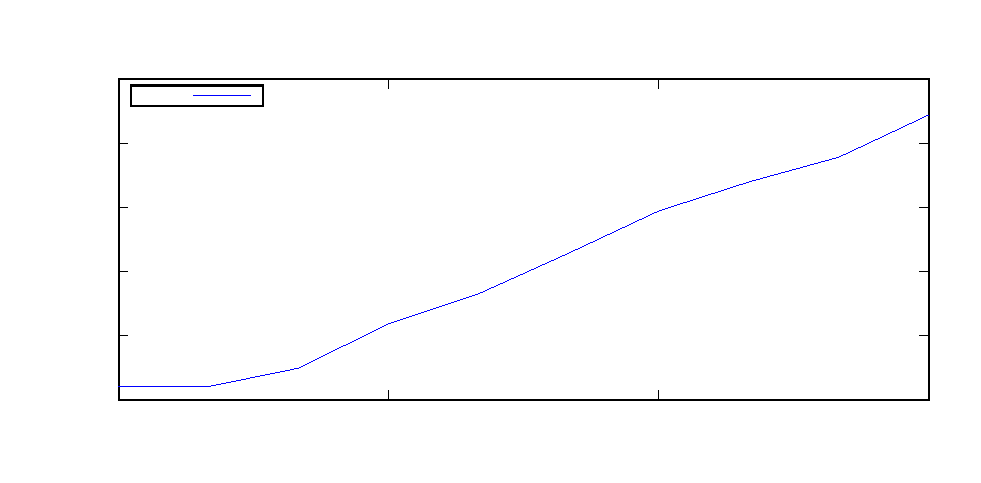
\includegraphics{problema3-peor-caso}}%
    \gplfronttext
  \end{picture}%
\endgroup

  \caption{Peor caso}
\end{figure}


\subsubsection{Mejor caso}

\begin{figure}[H]
  \centering
  % GNUPLOT: LaTeX picture with Postscript
\begingroup
  \makeatletter
  \providecommand\color[2][]{%
    \GenericError{(gnuplot) \space\space\space\@spaces}{%
      Package color not loaded in conjunction with
      terminal option `colourtext'%
    }{See the gnuplot documentation for explanation.%
    }{Either use 'blacktext' in gnuplot or load the package
      color.sty in LaTeX.}%
    \renewcommand\color[2][]{}%
  }%
  \providecommand\includegraphics[2][]{%
    \GenericError{(gnuplot) \space\space\space\@spaces}{%
      Package graphicx or graphics not loaded%
    }{See the gnuplot documentation for explanation.%
    }{The gnuplot epslatex terminal needs graphicx.sty or graphics.sty.}%
    \renewcommand\includegraphics[2][]{}%
  }%
  \providecommand\rotatebox[2]{#2}%
  \@ifundefined{ifGPcolor}{%
    \newif\ifGPcolor
    \GPcolorfalse
  }{}%
  \@ifundefined{ifGPblacktext}{%
    \newif\ifGPblacktext
    \GPblacktexttrue
  }{}%
  % define a \g@addto@macro without @ in the name:
  \let\gplgaddtomacro\g@addto@macro
  % define empty templates for all commands taking text:
  \gdef\gplbacktext{}%
  \gdef\gplfronttext{}%
  \makeatother
  \ifGPblacktext
    % no textcolor at all
    \def\colorrgb#1{}%
    \def\colorgray#1{}%
  \else
    % gray or color?
    \ifGPcolor
      \def\colorrgb#1{\color[rgb]{#1}}%
      \def\colorgray#1{\color[gray]{#1}}%
      \expandafter\def\csname LTw\endcsname{\color{white}}%
      \expandafter\def\csname LTb\endcsname{\color{black}}%
      \expandafter\def\csname LTa\endcsname{\color{black}}%
      \expandafter\def\csname LT0\endcsname{\color[rgb]{1,0,0}}%
      \expandafter\def\csname LT1\endcsname{\color[rgb]{0,1,0}}%
      \expandafter\def\csname LT2\endcsname{\color[rgb]{0,0,1}}%
      \expandafter\def\csname LT3\endcsname{\color[rgb]{1,0,1}}%
      \expandafter\def\csname LT4\endcsname{\color[rgb]{0,1,1}}%
      \expandafter\def\csname LT5\endcsname{\color[rgb]{1,1,0}}%
      \expandafter\def\csname LT6\endcsname{\color[rgb]{0,0,0}}%
      \expandafter\def\csname LT7\endcsname{\color[rgb]{1,0.3,0}}%
      \expandafter\def\csname LT8\endcsname{\color[rgb]{0.5,0.5,0.5}}%
    \else
      % gray
      \def\colorrgb#1{\color{black}}%
      \def\colorgray#1{\color[gray]{#1}}%
      \expandafter\def\csname LTw\endcsname{\color{white}}%
      \expandafter\def\csname LTb\endcsname{\color{black}}%
      \expandafter\def\csname LTa\endcsname{\color{black}}%
      \expandafter\def\csname LT0\endcsname{\color{black}}%
      \expandafter\def\csname LT1\endcsname{\color{black}}%
      \expandafter\def\csname LT2\endcsname{\color{black}}%
      \expandafter\def\csname LT3\endcsname{\color{black}}%
      \expandafter\def\csname LT4\endcsname{\color{black}}%
      \expandafter\def\csname LT5\endcsname{\color{black}}%
      \expandafter\def\csname LT6\endcsname{\color{black}}%
      \expandafter\def\csname LT7\endcsname{\color{black}}%
      \expandafter\def\csname LT8\endcsname{\color{black}}%
    \fi
  \fi
  \setlength{\unitlength}{0.0500bp}%
  \begin{picture}(7678.00,5280.00)%
    \gplgaddtomacro\gplbacktext{%
      \colorrgb{0.00,0.00,0.00}%
      \put(620,640){\makebox(0,0)[r]{\strut{}-1}}%
      \colorrgb{0.00,0.00,0.00}%
      \put(620,1448){\makebox(0,0)[r]{\strut{}0}}%
      \colorrgb{0.00,0.00,0.00}%
      \put(620,2256){\makebox(0,0)[r]{\strut{}1}}%
      \colorrgb{0.00,0.00,0.00}%
      \put(620,3063){\makebox(0,0)[r]{\strut{}2}}%
      \colorrgb{0.00,0.00,0.00}%
      \put(620,3871){\makebox(0,0)[r]{\strut{}3}}%
      \colorrgb{0.00,0.00,0.00}%
      \put(620,4679){\makebox(0,0)[r]{\strut{}4}}%
      \colorrgb{0.00,0.00,0.00}%
      \put(740,440){\makebox(0,0){\strut{}1x1,}}%
      \colorrgb{0.00,0.00,0.00}%
      \put(2328,440){\makebox(0,0){\strut{}63x63,}}%
      \colorrgb{0.00,0.00,0.00}%
      \put(3915,440){\makebox(0,0){\strut{}126x125,}}%
      \colorrgb{0.00,0.00,0.00}%
      \put(5503,440){\makebox(0,0){\strut{}188x188,}}%
      \colorrgb{0.00,0.00,0.00}%
      \put(7078,440){\makebox(0,0){\strut{}250x250,}}%
      \colorrgb{0.00,0.00,0.00}%
      \put(160,2659){\rotatebox{90}{\makebox(0,0){\strut{}Tiempo de ejecuci\'on [$mS$]}}}%
      \colorrgb{0.00,0.00,0.00}%
      \put(3909,140){\makebox(0,0){\strut{}$n$ (tama\~no del problema)}}%
      \csname LTb\endcsname%
      \put(3909,4979){\makebox(0,0){\strut{}Mejor caso}}%
    }%
    \gplgaddtomacro\gplfronttext{%
      \csname LTb\endcsname%
      \put(1100,4516){\makebox(0,0)[r]{\strut{}$t_n$}}%
    }%
    \gplbacktext
    \put(0,0){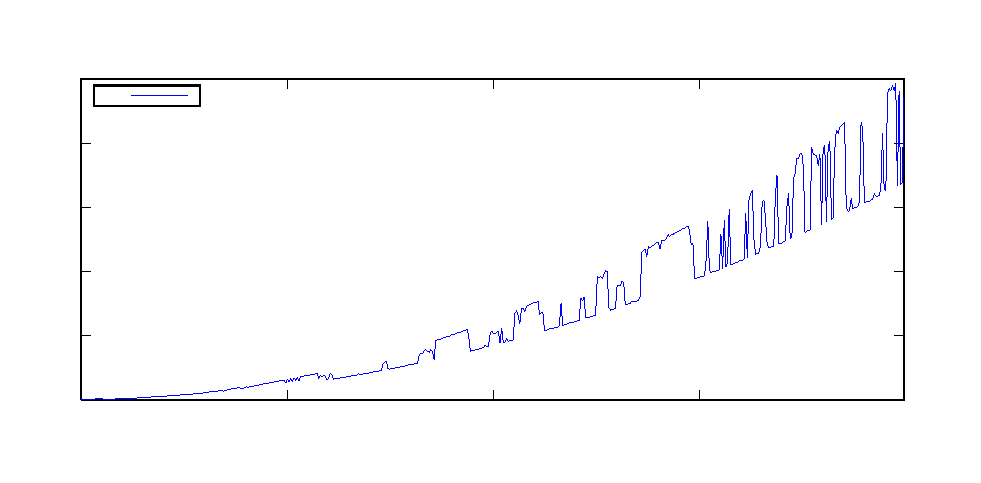
\includegraphics{problema3-mejor-caso}}%
    \gplfronttext
  \end{picture}%
\endgroup

  \caption{Mejor caso}
\end{figure}


\subsubsection{Instancias aleatorias}

\begin{figure}[H]
  \centering
  % GNUPLOT: LaTeX picture with Postscript
\begingroup
  \makeatletter
  \providecommand\color[2][]{%
    \GenericError{(gnuplot) \space\space\space\@spaces}{%
      Package color not loaded in conjunction with
      terminal option `colourtext'%
    }{See the gnuplot documentation for explanation.%
    }{Either use 'blacktext' in gnuplot or load the package
      color.sty in LaTeX.}%
    \renewcommand\color[2][]{}%
  }%
  \providecommand\includegraphics[2][]{%
    \GenericError{(gnuplot) \space\space\space\@spaces}{%
      Package graphicx or graphics not loaded%
    }{See the gnuplot documentation for explanation.%
    }{The gnuplot epslatex terminal needs graphicx.sty or graphics.sty.}%
    \renewcommand\includegraphics[2][]{}%
  }%
  \providecommand\rotatebox[2]{#2}%
  \@ifundefined{ifGPcolor}{%
    \newif\ifGPcolor
    \GPcolorfalse
  }{}%
  \@ifundefined{ifGPblacktext}{%
    \newif\ifGPblacktext
    \GPblacktexttrue
  }{}%
  % define a \g@addto@macro without @ in the name:
  \let\gplgaddtomacro\g@addto@macro
  % define empty templates for all commands taking text:
  \gdef\gplbacktext{}%
  \gdef\gplfronttext{}%
  \makeatother
  \ifGPblacktext
    % no textcolor at all
    \def\colorrgb#1{}%
    \def\colorgray#1{}%
  \else
    % gray or color?
    \ifGPcolor
      \def\colorrgb#1{\color[rgb]{#1}}%
      \def\colorgray#1{\color[gray]{#1}}%
      \expandafter\def\csname LTw\endcsname{\color{white}}%
      \expandafter\def\csname LTb\endcsname{\color{black}}%
      \expandafter\def\csname LTa\endcsname{\color{black}}%
      \expandafter\def\csname LT0\endcsname{\color[rgb]{1,0,0}}%
      \expandafter\def\csname LT1\endcsname{\color[rgb]{0,1,0}}%
      \expandafter\def\csname LT2\endcsname{\color[rgb]{0,0,1}}%
      \expandafter\def\csname LT3\endcsname{\color[rgb]{1,0,1}}%
      \expandafter\def\csname LT4\endcsname{\color[rgb]{0,1,1}}%
      \expandafter\def\csname LT5\endcsname{\color[rgb]{1,1,0}}%
      \expandafter\def\csname LT6\endcsname{\color[rgb]{0,0,0}}%
      \expandafter\def\csname LT7\endcsname{\color[rgb]{1,0.3,0}}%
      \expandafter\def\csname LT8\endcsname{\color[rgb]{0.5,0.5,0.5}}%
    \else
      % gray
      \def\colorrgb#1{\color{black}}%
      \def\colorgray#1{\color[gray]{#1}}%
      \expandafter\def\csname LTw\endcsname{\color{white}}%
      \expandafter\def\csname LTb\endcsname{\color{black}}%
      \expandafter\def\csname LTa\endcsname{\color{black}}%
      \expandafter\def\csname LT0\endcsname{\color{black}}%
      \expandafter\def\csname LT1\endcsname{\color{black}}%
      \expandafter\def\csname LT2\endcsname{\color{black}}%
      \expandafter\def\csname LT3\endcsname{\color{black}}%
      \expandafter\def\csname LT4\endcsname{\color{black}}%
      \expandafter\def\csname LT5\endcsname{\color{black}}%
      \expandafter\def\csname LT6\endcsname{\color{black}}%
      \expandafter\def\csname LT7\endcsname{\color{black}}%
      \expandafter\def\csname LT8\endcsname{\color{black}}%
    \fi
  \fi
  \setlength{\unitlength}{0.0500bp}%
  \begin{picture}(7678.00,5280.00)%
    \gplgaddtomacro\gplbacktext{%
      \colorrgb{0.00,0.00,0.00}%
      \put(740,640){\makebox(0,0)[r]{\strut{}$10^{0}$}}%
      \colorrgb{0.00,0.00,0.00}%
      \put(740,2660){\makebox(0,0)[r]{\strut{}$10^{1}$}}%
      \colorrgb{0.00,0.00,0.00}%
      \put(740,4679){\makebox(0,0)[r]{\strut{}$10^{2}$}}%
      \colorrgb{0.00,0.00,0.00}%
      \put(860,440){\makebox(0,0){\strut{}1x1,}}%
      \colorrgb{0.00,0.00,0.00}%
      \put(3012,440){\makebox(0,0){\strut{}2x2,}}%
      \colorrgb{0.00,0.00,0.00}%
      \put(5165,440){\makebox(0,0){\strut{}4x3,}}%
      \colorrgb{0.00,0.00,0.00}%
      \put(7317,440){\makebox(0,0){\strut{}5x5,}}%
      \colorrgb{0.00,0.00,0.00}%
      \put(160,2659){\rotatebox{90}{\makebox(0,0){\strut{}Tiempo de ejecuci\'on [$mS$]}}}%
      \colorrgb{0.00,0.00,0.00}%
      \put(4088,140){\makebox(0,0){\strut{}$n$ (tama\~no del problema)}}%
      \csname LTb\endcsname%
      \put(4088,4979){\makebox(0,0){\strut{}Instancias aleatorias}}%
    }%
    \gplgaddtomacro\gplfronttext{%
      \csname LTb\endcsname%
      \put(1220,4516){\makebox(0,0)[r]{\strut{}$t_n$}}%
    }%
    \gplbacktext
    \put(0,0){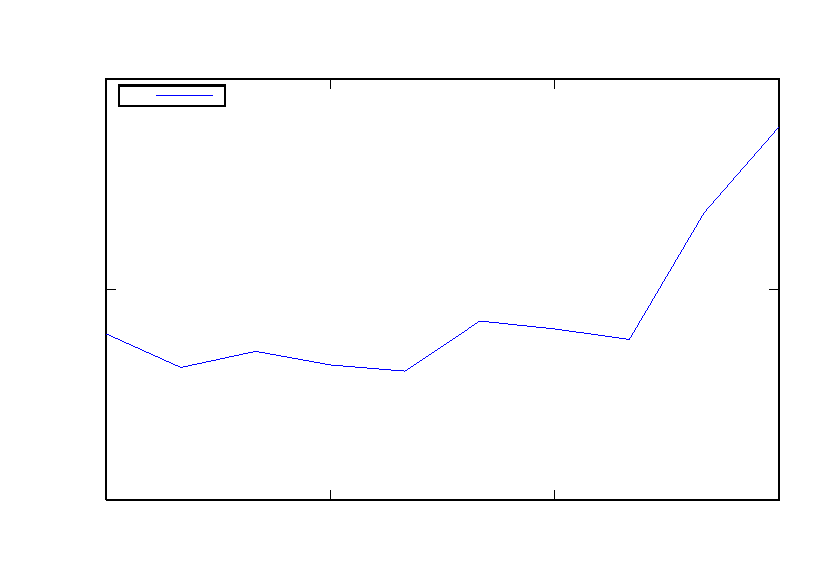
\includegraphics{problema3-instancias-aleatorias}}%
    \gplfronttext
  \end{picture}%
\endgroup

  \caption{Instancias aleatorias}
\end{figure}


%%%%%%%%%%%%%%%%%%%%%%%%%%%%%%%%%%%%%%%%%%%%%%%%%%%%%%%%%%%%%%%%%%%%%%%%%%%%%%%
%% Conclusiones                                                              %%
%%%%%%%%%%%%%%%%%%%%%%%%%%%%%%%%%%%%%%%%%%%%%%%%%%%%%%%%%%%%%%%%%%%%%%%%%%%%%%%


\newpage

\section{Conclusiones}

Observamos que para los tres problemas estudiados, las cotas de complejidad teórica se condicen con los experimentos computacionales realizados.

Extraemos las siguientes conclusiones para los tres problemas:

\begin{itemize}
    \item{Las mediciones de tiempo de mejor caso, peor caso e instancias aleatorias respetan las cotas de complejidad temporal correspondientes.}
    \item{El tiempo de ejecución del mejor caso es inferior al del peor caso para instancias a partir de cierto tamaño.}
    \item{El tiempo de ejecución para instancias aleatorias es superior al del mejor caso e inferior al del peor caso para problemas a partir de cierto tamaño.}
\end{itemize}


%%%%%%%%%%%%%%%%%%%%%%%%%%%%%%%%%%%%%%%%%%%%%%%%%%%%%%%%%%%%%%%%%%%%%%%%%%%%%%%
%% Código fuente para el problema 1                                          %%
%%%%%%%%%%%%%%%%%%%%%%%%%%%%%%%%%%%%%%%%%%%%%%%%%%%%%%%%%%%%%%%%%%%%%%%%%%%%%%%


\newpage

\begin{appendices}

\section{Código fuente para el problema 1}


\subsection{problema1.h}

\verbatiminput{../src/problema1/problema1.h}


\subsection{problema1.cpp}

\verbatiminput{../src/problema1/problema1.cpp}


%%%%%%%%%%%%%%%%%%%%%%%%%%%%%%%%%%%%%%%%%%%%%%%%%%%%%%%%%%%%%%%%%%%%%%%%%%%%%%%
%% Código fuente para el problema 1                                          %%
%%%%%%%%%%%%%%%%%%%%%%%%%%%%%%%%%%%%%%%%%%%%%%%%%%%%%%%%%%%%%%%%%%%%%%%%%%%%%%%


\newpage

\section{Código fuente para el problema 2}


\subsection{problema2.h}

\verbatiminput{../src/problema2/problema2.h}


\subsection{problema2.cpp}

\verbatiminput{../src/problema2/problema2.cpp}


%%%%%%%%%%%%%%%%%%%%%%%%%%%%%%%%%%%%%%%%%%%%%%%%%%%%%%%%%%%%%%%%%%%%%%%%%%%%%%%
%% Código fuente para el problema 3                                          %%
%%%%%%%%%%%%%%%%%%%%%%%%%%%%%%%%%%%%%%%%%%%%%%%%%%%%%%%%%%%%%%%%%%%%%%%%%%%%%%%


\newpage

\section{Código fuente para el problema 3}


\subsection{problema3.h}

\verbatiminput{../src/problema3/problema3.h}


\subsection{problema3.cpp}

\verbatiminput{../src/problema3/problema3.cpp}


\end{appendices}

\end{document}